\begin{figure}[h]
  % adapted from https://tex.stackexchange.com/a/122813/316176
  \captionsetup[subfigure]{justification=raggedright}
  \begin{minipage}{0.7\textwidth}

    \begin{minipage}{0.04\textwidth}~\end{minipage}%
    \begin{minipage}{0.44\textwidth}
      \centering
      \itshape
      \textbf{unlimited} beneficial mutations
    \end{minipage}%
    \begin{minipage}{0.34\textwidth}
      \centering
      \itshape
      \textbf{single} beneficial mutation
    \end{minipage}

    ~\vspace{-1.5ex}

    % Top subfigure
    \begin{subfigure}[b]{\linewidth}
      \begin{minipage}{0.88\textwidth}
        \begin{minipage}{0.53\textwidth}
          \includegraphics[height=2.9cm, trim={0cm 0.2cm 3.5cm 0.8cm}, clip]{binder/binder-wse-5050-spatial2d-32atile-infben-traits.ipynb/binder/teeplots/wse-5050-spatial2d-32atile-infben-traits/errorbar=ci+hue=genotype+num-abm=(inf,)+style=genotype+viz=size-fixation-areaplot+x=population-size+y=fixation-probability+ext=.pdf}%
        \end{minipage}%
        \begin{minipage}{0.47\textwidth}
          \includegraphics[height=2.9cm, trim={1.3cm 0.2cm 3.5cm 0.8cm}, clip]{binder/binder-wse-5050-spatial2d-32atile-infben-traits.ipynb/binder/teeplots/wse-5050-spatial2d-32atile-infben-traits/errorbar=ci+hue=genotype+num-abm=(1.0,)+style=genotype+viz=size-fixation-areaplot+x=population-size+y=fixation-probability+ext=.pdf}
        \end{minipage}
      \end{minipage}%
      \hspace{-3ex}%
      \begin{minipage}{0.12\textwidth}
        \raggedright
        \caption{\footnotesize 32 agents per PE\\~\\~\\}
        \label{fig:wse-inf-one:32}
      \end{minipage}%
    \end{subfigure}%

    % Bottom subfigure - Adjusted layout to match the top
    \begin{subfigure}[b]{\linewidth}
      \begin{minipage}{0.88\textwidth}
        \begin{minipage}{0.53\textwidth}
          \includegraphics[height=2.9cm, trim={0cm 0.2cm 3.7cm 0.8cm}, clip]{binder/binder-wse-5050-spatial2d-2048atile-infben-traits.ipynb/binder/teeplots/wse-5050-spatial2d-2048atile-infben-traits/errorbar=ci+hue=genotype+num-abm=(inf,)+style=genotype+viz=size-fixation-areaplot+x=population-size+y=fixation-probability+ext=.pdf}%
        \end{minipage}%
        \begin{minipage}{0.47\textwidth}
          \includegraphics[height=2.9cm, trim={1.3cm 0.2cm 3.7cm 0.8cm}, clip]{binder/binder-wse-5050-spatial2d-2048atile-infben-traits.ipynb/binder/teeplots/wse-5050-spatial2d-2048atile-infben-traits/errorbar=ci+hue=genotype+num-abm=(1.0,)+style=genotype+viz=size-fixation-areaplot+x=population-size+y=fixation-probability+ext=.pdf}
        \end{minipage}
      \end{minipage}%
      \hspace{-3ex}%
      \begin{minipage}{0.1\textwidth}
        \caption{\footnotesize 2,048 agents per PE\\~\\~\\}
        \label{fig:wse-inf-one:2048}
      \end{minipage}%
    \end{subfigure}%

~\vspace{-1.2ex}

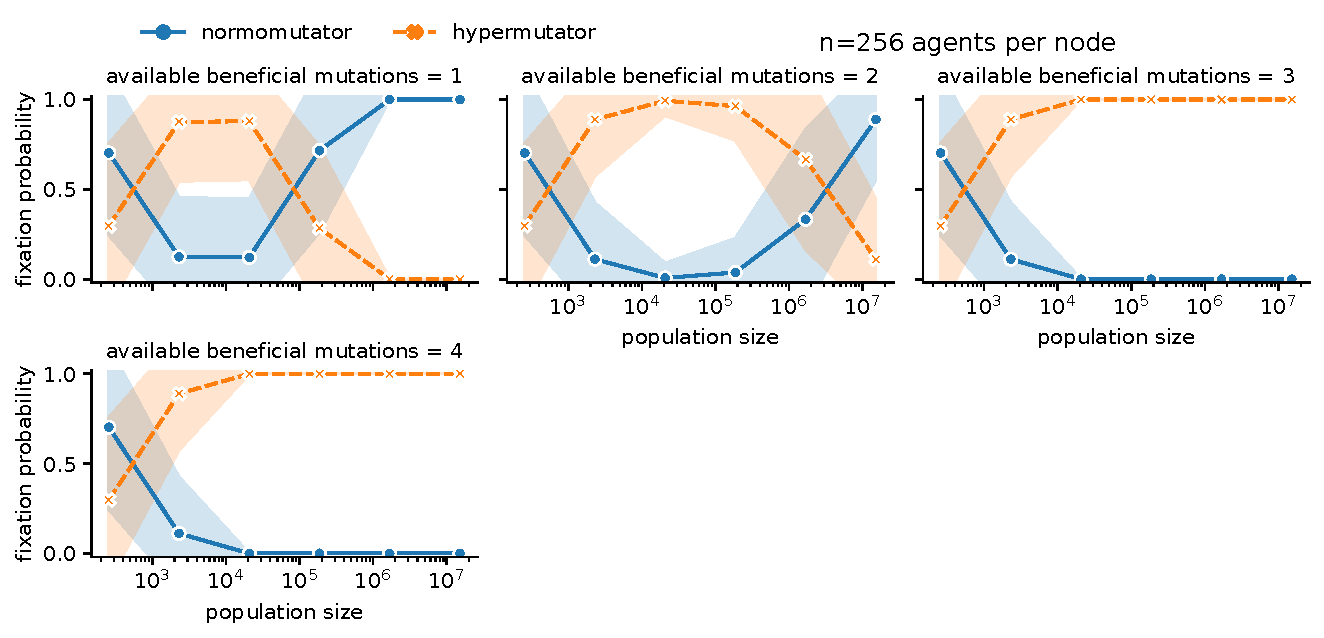
\includegraphics[width=0.9\textwidth, trim={0cm 4.7cm 6.2cm 0cm}, clip]{binder/binder-wse-5050-spatial2d-2048atile-infben-traits.ipynb/binder/teeplots/wse-5050-spatial2d-2048atile-infben-traits/col=available-beneficial-mutations+errorbar=sd+hue=genotype+kind=line+style=genotype+viz=relplot+x=population-size+y=fixation-probability+ext=}

  \end{minipage}%
  \begin{minipage}{0.3\textwidth}
    \caption{%
      \textbf{Restricted adaptive potential favors nonmutators in large populations.}
      \footnotesize
      Area plots compare mutator versus nonmutator fixation probabilities across surveyed population sizes.
      When adaptive potential is unlimited (left column), mutators are strongly favored in large populations, owing to their capacity to more rapidly discover beneficial mutations.
      Right column shows fixation outcomes across population sizes, with adaptive potential restricted to just one beneficial mutation.
      As before, mutators gain favor in intermediate population sizes.
      However, under the adaptation-restricted regime, nonmutators regain favor at very large population sizes.
      Top panel, \ref{fig:wse-inf-one:32}, shows results with subpopulation size of 32 agents per PE, scaling population size up to 23.9 million.
      Bottom panel, \ref{fig:wse-inf-one:2048}, reports 2,048 agents per PE with population sizes up to 1.5 billion.
      Experiments were conducted on WSE with counter-based genome model, using populations initialized with a 50/50 mix of non- and mutators.
      Error bands indicate bootstrapped 95\% confidence intervals.
      Supplementary Figure \ref{fig:fixheat-wse-altatile} details results in a tabular format.
    }
    \label{fig:wse-inf-one}
  \end{minipage}
\end{figure}
